% Compile with XeLaTeX or LuaLaTeX
\documentclass[11pt,a4paper,oneside]{article}
%\usepackage[latin1]{inputenc}
%\usepackage[utf8]{inputenc}
\usepackage{graphicx}
%\usepackage{epsfig}
\usepackage{epstopdf}
%\usepackage{subfigure}
\usepackage{caption}
\usepackage{subcaption}
\usepackage{setspace}
\usepackage{amsmath}
\usepackage{amsfonts}
\usepackage{amsthm}
\usepackage{algorithm}
\usepackage{algorithmic}
\usepackage{array}
\usepackage{gensymb}
\usepackage{rotating}
\usepackage{lettrine}
%\usepackage{sectsty}

\newcommand{\matlabel}[2]{% \matlabel{<label>}{<stuff>}
  \begin{array}{@{}c@{}} \mbox{\small$#1$} \\ #2 \end{array}
}

\newtheorem{theorem}{Theorem}
\newtheorem{definition}{Definition}
\newtheorem{lemma}{Lemma}

%\usepackage[tmargin=1in,bmargin=1in,lmargin=1.25in,rmargin=1.25in]{geometry}
\usepackage[pdfauthor={Wissem Allouchi},pdftitle={Combined camera and microphone calibration},pdfsubject={Master semester project},bookmarks=true,linkcolor=black,colorlinks=true,urlcolor=blue,citecolor=blue]{hyperref}

\renewcommand{\algorithmicrequire}{\textbf{Input:}}
\renewcommand{\algorithmicensure}{\textbf{Output:}}

\newcommand{\submissionDay}{05}
\newcommand{\submissionMonth}{June}
\newcommand{\submissionYear}{2015}
\newcommand{\submissionDate}{\sffamily \submissionMonth ~\submissionDay,~\submissionYear}
\newcommand{\authorOfThesis}{Wissem Allouchi}
\newcommand{\typeOfThesis}{Semester project report}


\newcommand{\titleOfThesis}{\sffamily Calibration algorithms for audio-visual wearable devices}
\newcommand{\supervisorOne}{\sffamily Ivan Dokmanic�}
\newcommand{\supervisorTwo}{\sffamily Juri Ranieri�}
\newcommand{\supervisorThree}{Prof. Martin Vetterli}


\begin{document}
\newcolumntype{C}{>{\(\displaystyle}c<{\)}@{}} 
\newcolumntype{L}{>{\(\displaystyle}l<{\)}@{}} 
\newcolumntype{R}{>{\(\displaystyle}r<{\)}@{}}

\newcommand{\titlePage}{

\thispagestyle{empty}
\begin{center}
	\Large { \sffamily \'{E}cole polytechnique f\'{e}d\'{e}rale de Lausanne}\\[2mm]
	   
\includegraphics[width=3cm]{images/epfl_logo.eps}\\[1mm]
	%	
\includegraphics[width=3cm]{images/epfl_logo_grey.eps}\\[1mm]
		\large { \sffamily School of Computer and Communication Sciences (IC)}\\[1mm]
	\large { \sffamily Laboratory of Audiovisual Communications}\\[1mm]
	
\includegraphics[width=3cm]{images/lcav_logo_320x180.jpg}\\[1mm]
	
	\vspace{2cm}
	\doublespacing
	{\Huge \sffamily \textsc{\titleOfThesis}}\\
	\singlespacing
	\vspace{2cm}
	{\LARGE \sffamily {\authorOfThesis}}\\
	\singlespacing
	{\large \sffamily {\typeOfThesis}}\\
	
	\vfill
	\parbox{1cm}{
  		\begin{large}
    			\begin{tabbing}
      			\sffamily Supervisor: \hspace{2cm}  
        			\=\supervisorOne\\[2mm]
				\>\supervisorTwo\\[2mm]
				\>\supervisorThree\\[2mm]
      			\sffamily Submission Date: 
        		\>\submissionDate\\[2mm]
    			\end{tabbing}
  		\end{large}
	}\\
\end{center}
\clearpage
}

%%%%%%%%%%%%%%%%%%%%%%%%%%%%%%%%%%%%%%%%%%%%%%%%%%%%%%%%%%%%%%%%%%%%%
\titlePage
%\thispagestyle{empty}\ \clearpage
%\titlePage
%%%%%%%%%%%%%%%%%%%%%%%%%%%%%%%%%%%%%%%%%%%%%%%%%%%%%%%%%%%%%%%%%%%%%


\tableofcontents
\section{Introduction}
Stuff \cite{fuchs2011}
\subsection{More stuff}
\begin{figure}[htb]%
\centering
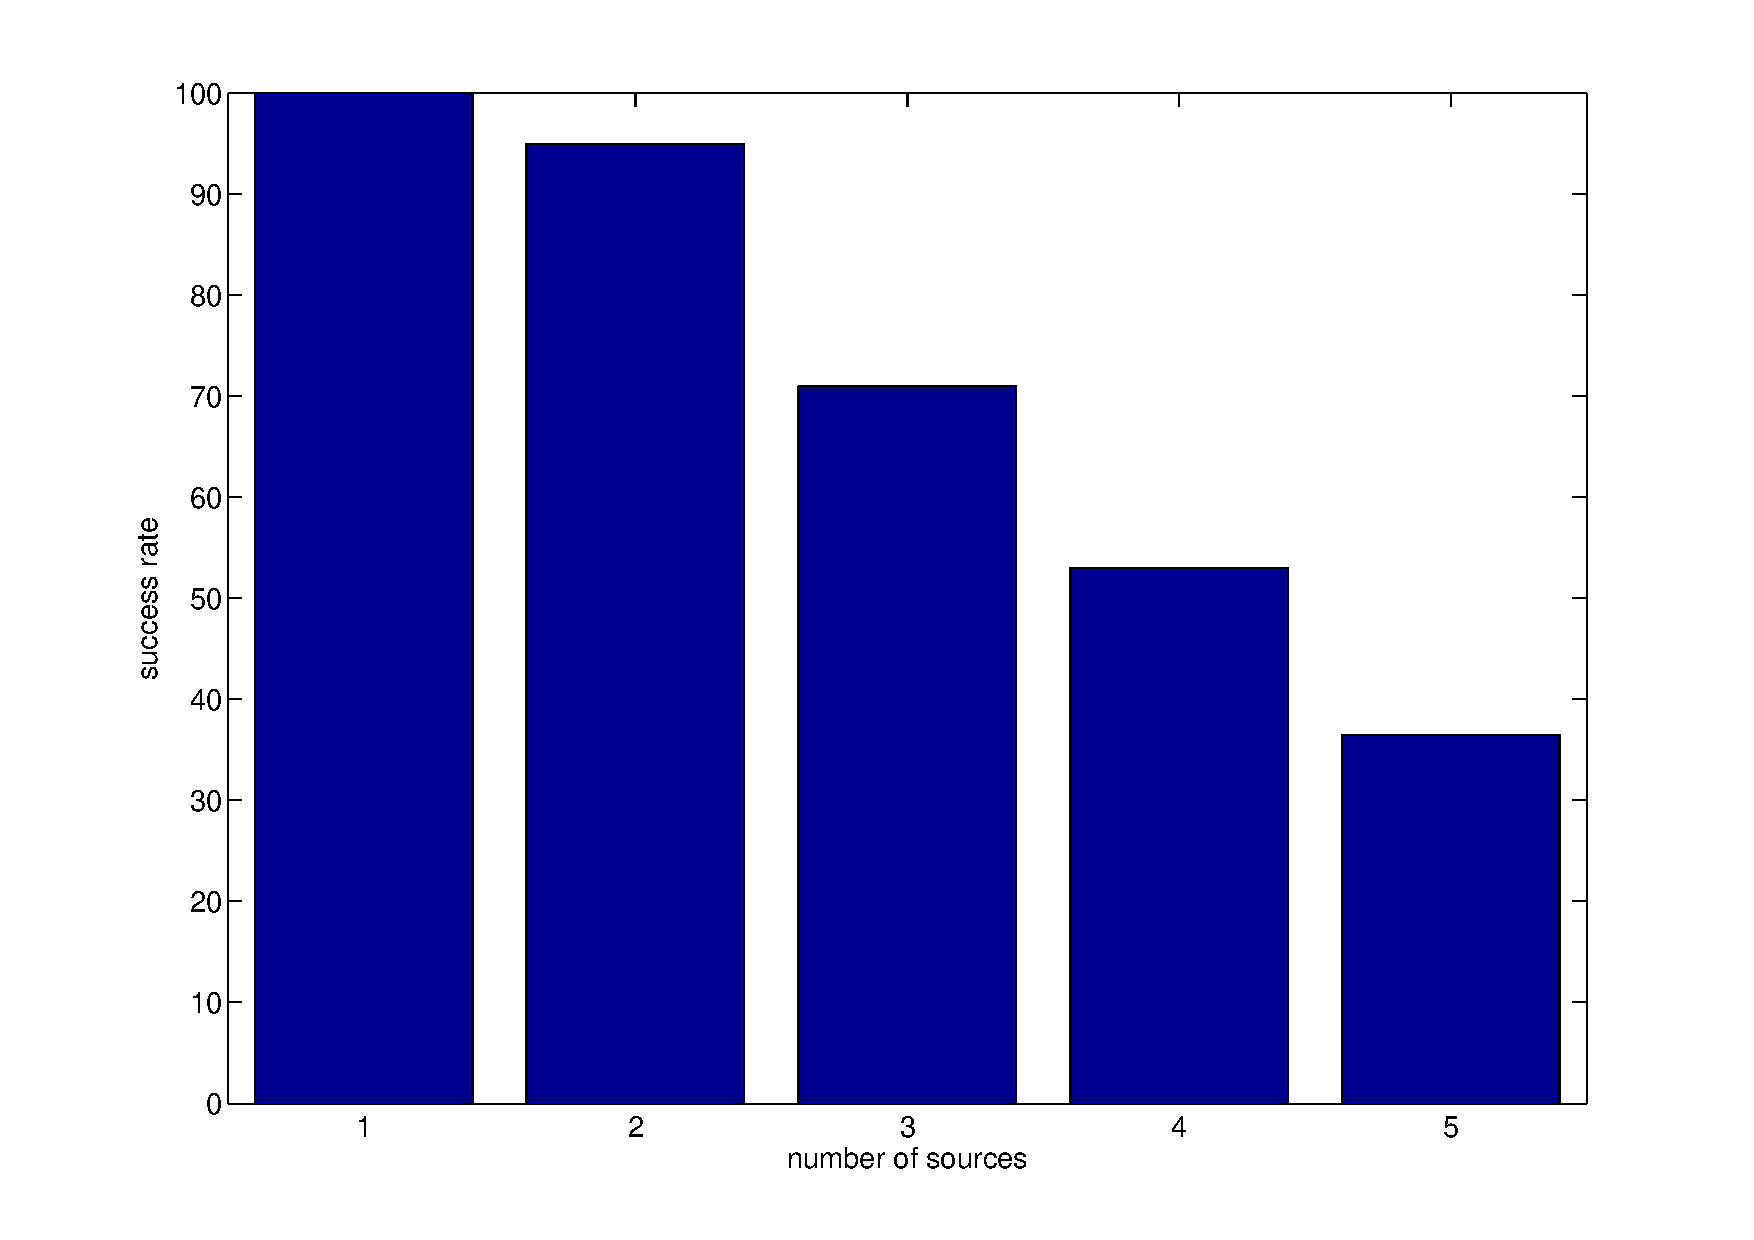
\includegraphics[width=0.8\columnwidth]{images/success_one_mic.pdf}%
\caption{Average success rate of localization using one microphone.}%
\label{onemicgauss}%
\end{figure}
%\include{approach}


\clearpage
%bibliography
\bibliographystyle{plain}
\bibliography{MasterProj}
\addcontentsline{toc}{section}{References}

\end{document}